\documentclass{vhdl-assignment}

\title{Assignment 7}
\date{2023}

\begin{document}
\maketitle
\thispagestyle{fancy}

\begin{problem}{}
    Use Behavioral model to design circuits.
    Simulate your designs on ModelSim.
    Create code coverage report, and waveform.
    Screenshot your results

    \subsection*{1. Encoder 8-to-3}
    \begin{figure}[H]
        \centering
        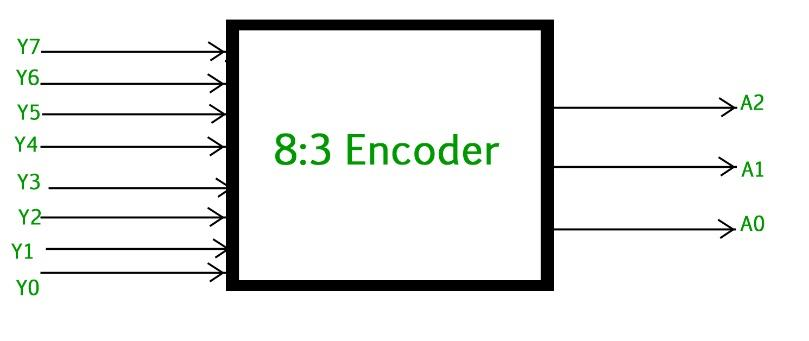
\includegraphics{assets/8_3_Encoder.jpg}
    \end{figure}

    \subsection*{2. Majority 4 bit circuit}

    \subsection*{3. BCD to 7-segment Decoder}
    \begin{figure}[H]
        \centering
        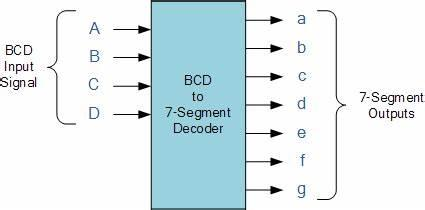
\includegraphics{assets/BCD_7_segment_Decoder.jpg}
    \end{figure}

    \subsection*{4. Flip Flops: D-FF, T-FF, SR-FF, JK-FF}
    \begin{enumerate}
        \item Use Synchronous reset.
        \item Use Asynchronous reset.
    \end{enumerate}

    How does these synthesis (Lecture 4)    
\end{problem}

\begin{problem}{Answer the questions}
    Describe the initial statement and always statement in Behavioral Verilog.
\end{problem}

\end{document}